\documentclass[spanish,11pt,letterpaper]{article}

\usepackage[spanish]{babel}
\usepackage[utf8]{inputenc}
\usepackage{authblk}
\usepackage{amsmath}
\usepackage{amssymb}
\usepackage{amsthm}
\usepackage[margin=1in]{geometry}
\usepackage{graphicx}
\usepackage{hyperref}
% \usepackage{listings}
% \usepackage{xcolor}

\renewcommand{\vec}[1]{\mathbf{#1}}
\DeclareMathOperator*{\argmax}{arg\,max}
\decimalpoint

\title{{\Huge Is this Loss?}\\
Sistema de reconocimiento de objetos en imágenes}
\author{Hernández Chiapa David Felipe\\
López García Gilberto Isaac}
\affil{Facultad de Ciencias\\Universidad Nacional Autónoma de México}
\date{\small\today}

\begin{document}

\maketitle

\section{Introducción}

El reconocimiento de objetos o patrones en imágenes siempre ha sido un reto para el ser humano, ya sea que se
vea el rostro de alguna deidad en el tronco de un árbol o alguna forma geométrica irregular al fondo de una taza
de té, pero hay veces que ciertas personas ven cierto patrón en alguna imagen y otras no, haciendo que nos
preguntemos si el patrón que, según nosotros, estamos viendo realmente está ahí o simplemente estamos perdiendo la cabeza. En otras
palabras, la detección de ciertos patrones en imágenes puede llegar a ser complicada, entonces surge la
pregunta, ¿existirá la manera de automatizar la detección de patrones?

En este escrito expondremos una manera de tratar de solucionar una instancia muy particular de este tipo de problemas usando redes neuronales convolucionales.

\section{Descripción del problema}

En la red existen cantidades colosales de imágenes de todo tipo, como caricaturas, motivacionales, científicas,
etcétera. Un subconjunto de todas esas imágenes es conocido como ``memes'', los cuales son imágenes que se burlan
de algún tema o situación, sin importar cual sea este.

En el año 2008 un caricaturista humorístico se salió totalmente de su estilo al
publicar un cómic donde se ilustra un momento difícil de su vida (ver Figura ~\ref{fig:loss}).
Tras recibir muchas críticas, el cómic se viralizó y con el tiempo los usuarios del internet
convirtieron esa deprimente caricatura en un meme, creando la famosa broma
`Is this Loss?'\cite{loss},
la cual consiste en generar una imagen divida en cuatro secciones siguiendo el patrón de la
caricatura original, es decir, en el primer cuadro debe haber algo que asemeje a una persona parada, en el
segundo y tercero a dos personas y en el cuarto a una persona parada y una acostada, y que otros
usuarios puedan identificar dicho patrón.

Por la naturaleza del meme, se generó una cantidad impresionante de ediciones o `edits' del mismo,
y en algunas de ellas es sorprendentemente difícil saber si realmente corresponde al patrón o no, pues
los usuarios pueden ser muy creativos y crear `edits' abstractos con figuras
que no tienen nada que ver unas con las otras, o muy sutiles con imágenes similares seleccionadas y
ordenadas específicamente para recrear el patrón.

Lo que se busca aquí es ver si una red neuronal puede identificar `edits' de manera precisa, algo que
ya se sabe puede ser difícil para el ser humano.

% ¿Por qué no un algoritmo ad-hoc?
Se eligió usar una red neuronal sobre algún algoritmo porqué las redes han mostrado un mejor desempeño en este tipo de procesamiento, i.e.
reconocimiento de patrones, mientras que diseñar un algoritmo para este tipo de problemas puede llegar a ser muy complicado, en especial por el
manejo de imágenes, ya que los `edits', del meme que intentaremos clasificar, suelen ser muy irregulares.

\section{Redes Neuronales Convolucionales\cite{lecun}}

Las redes convolucionales combinan tres ideas arquitectónicas para asegurar cierto
grado de invariancia ante desplazamiento, reescalamiento y distorción: campos
receptivos locales (también llamados en la literatura filtros o \textit{kernels}),
pesos compartidos, y submuestreo espacial o temporal%
\footnote{En inglés, \textit{local receptive fields}, \textit{shared weights},
\textit{spatial or temporal sub-sampling}.}.

La estructura general de una red neuronal convolucional consiste de:
\begin{itemize}
  \item Capa de convolución donde se realiza la detección de características.
  \item Capa de pooling donde se extraen las características importantes.
  \item Posiblemente más capas de convolución y pooling para extraer características
  más complejas.
  \item Un clasificador que asigna una categoría a la entrada en base a las
  características encontradas.
\end{itemize}

\subsection{Capa de convolución}

Con los campos receptivos se extraen características simples en localidades
pequeñas que en capas posteriores
son combinadas para detectar características de orden superior. Estas características
pueden estar en distintas posiciones (espaciales o temporales) en las muestras
de entrada por lo que se elige tener campos receptivos en distintas posiciones
que comparten el mismo conjunto de pesos\footnote{Por decirlo de otra forma, un
mismo campo receptivo se aplica a todo un ejemplar en distintas posiciones.}, y
se obtiene un mapa de características o \textit{feature map}. Esta operación es
una convolución.

Por cada campo receptivo se obtiene un mapa de características, el conjunto de
estos mapas forman una capa de convolución completa.

Los mapas de caracerísticas tienen la propiedad de preservar las posiciones
relativas de características. Una vez que una característica se ha detectado,
su posición exacta se vuelve menos importante. Solo su posición relativa a otras
características es relevante.

\subsection{Pooling}

Como la posición exacta de las características es irrelevante para identificar
un patrón más complejo, e inclusive dañina pues puede variar entre muestras, se
aplican capas de submuestreo que reduce el tamaño de los mapas de características
preservando la información importante y reduciendo la sensibilidad de la salida
a desplazamientos y distorsiones.

La preservación de estas características importantes puede realizarse promediando
valores locales (contiguos) en los mapas de características (manteniendo posiciones
relativas entre características) que es \textit{average sub-sampling}, o manteniendo
los valores máximos en localidades contiguas que es \textit{max pooling}.

\textit{Max pooling} ha demostrado dar mejores resultados en la praćtica que
\textit{average sub-sampling}\cite{pooling}. Además, localidades contiguas que se traslapan
no son una mejora significativa sobre aquellas que no se traslapan, estás
últimas reducen aún más el tamaño de los mapas de características.

\subsection{Perceptrón Multicapa}

Una vez extraídas las múltiples características relevantes, con una reducción
de dimensionalidad, y posiblemente combinadas para detección de características
más complejas agregando capas de convolución y pooling, se puede utilizar un
clasificador para determinar la categoría a la que pertenece un ejemplar.
Generalmente un perceptrón multicapa o red \textit{feed-forward}.

\subsection{Espacio de Hipótesis}

Las redes neuronales convolucionales para reconocimiento de objetos en imágenes
son funciones que asignan a sus entradas, imágenes de $N$ pixeles de alto por $M$
pixeles de alto, una etiqueta o categoría, las imágenes se pueden representar
como tensores de orden $C$, esto es, elementos del espacio
$\mathbb{R}^{N\times M\times C}$, donde $C$ es el número de canales, que puede ser
1 si se trabaja en escala de grises, 3 si se trabaja con colores (como RGB), etc.

Las entradas de estos tensores toman valores en un conjunto finito: $\{0,\ldots,255\}$,
pero dado que se requiere hacer operaciones aritméticas con sus valores de entrada
es conveniente verlos como números reales. Si tenemos entonces $K$ categorías
distintas, existe un total de $K^{256^{NMC}}$ funciones de clasificación para
imágenes, pero de la misma forma que con los árboles de decisión, existen múltiples
redes convolucionales capaces de computar la misma función.

Nuestro espacio de hipótesis son todas las redes convolucionales para clasficación
de imágenes en resolución $250 \times 250$ con 1 canal en escala de grises y 3
canales en RGB, con $K = 2$ categorías. Esto es al menos
\[ 2^{256^{250^2}} \text{  y  } 2^{256^{250^2 \cdot 3}}\]
redes convolucionales respectivamente.

\subsection{Ventajas y desventajas}

La principal ventaja de las redes convolucionales es que son capaces de encontrar
características importantes en los datos por cuenta propia durante el entrenamiento,
aprovechándose de la existencia de correlaciones locales entre los datos. Poseen
un alto grado de invariancia ante cambios o distorciones en los datos pues
se extraen características locales y se preserva la relación espacial o temporal
entre ellas. Debido a que un mismo campo receptivo se aplica a distintas zonas de
los datos hay una reducción en el número de parámetros libres que se
deben ajustar en el entrenamiento\cite{haykin}.

Entre las desventajas está el alto poder computacional requerido. Aunque hay una
reducción de dimensionalidad al pasar de la entrada a mapas de características y
aplicar pooling, la entrada suele tener dimensiones altas como se aprecia en la subsección
anterior, por lo que capas convolucionales completas pueden tener un cantidad
relativamente pequeña de mapas relativamente grandes, y aunque la dimensión sigue
decreciendo en capas subsecuentes, el número de mapas sigue aumentando, entonces
hay mayor cantidad de parámetros a ajustar al haber gran cantidad de campos receptivos,
además del perceptrón multicapa que realiza la clasificación. También se requiere
de un conjunto de datos para entrenamiento extenso para obtener buenos resutlados.

En la práctica se han visto casos de redes convolucionales con un desempeño pobre
ante cambios pequeños como cambios de iluminación en fotos, por lo que se podría
pensar que tienen una tendencia a sobreajustarse y no entender o generalizar las
características de los objetos que están procesando\cite{limitations}.

\section{Propuesta e implementación}

Para la clasificación de imágenes en nuestras dos categorías \texttt{loss\_edit}
y \texttt{not\_loss}, donde la primera son `edits' de Loss y la segunda memes
variados, utilizaremos una red neuronal convolucional, la entrenaremos para que
aprenda a determinar qué imágenes o memes son `edits' de Loss, los cuales siguen
un patrón muy específico, imitando el cómic Loss%
\footnote{\url{http://cad-comic.com/comic/loss/}} (ver Figura ~\ref{fig:loss}).

Una primera aproximación sería tratar de clasificar imágenes en escala de grises
pues lo que importa para la clasificación es reconocer los objetos que aparecen
en ellas y comparar su orientación con el patrón buscado. Por desgracia existen
`edits' basados en la distinción de colores (ver Figura ~\ref{fig:color}), por lo
que podría ser más preciso trabajar con colores (por si distintos colores se
``funden'' en la escala de grises por tener un tono similar).

Una idea que surgió poco después fue no trabajar con las imágenes originales, sino
con las aristas. Usando el Algoritmo de Canny para extraer las aristas, es decir,
las siluetas de las formas o polígonos, se podría facilitar el trabajo de
clasificación, pero al intentar esto nos dimos cuenta que podría no ayudar o
incluso dificultar la tarea de nuestros modelos. Más adelante se hablará de los problemas
econtrados que nos llevaron a descartar esta idea en el trabajo.

\begin{figure}[h]
\centering
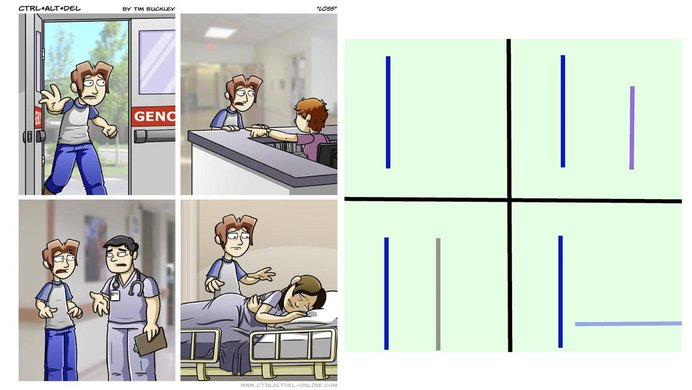
\includegraphics[width=0.8\textwidth]{lossminimal}
\caption{Cómic original (izq.), patrón buscado (der.)}
\label{fig:loss}
\end{figure}

Es importante aclarar que estas imágenes conservan un patrón muy específico, por
lo que no tendría sentido realizar modificaciones como reflexiones o rotaciones
a las imágenes pues la orientación de los objetos es clave en los `edits'.

\subsection{Datos}

El conjunto de datos consiste de una colección de 1735 imágenes, 1304 para
entrenamiento (con 558 `edits') y 431 para verificación (con 185 `edits'), divididas
en nuestras ya mencionadas dos categorías.

Los memes variados se obtuvieron de la colección personal de memes de los
desarrolladores, obtenidas con el paso del tiempo ya sea descargándolas de
distintos sitios de internet como redes sociales, chats de WhatsApp, Messenger,
etc., mientras que los `edits' de Loss se descargaron principalmente de la galería
de \textsf{KnowYourMeme.com}\footnote{\url{http://knowyourmeme.com/memes/loss/photos}} y
\textsf{Google Images} (que son miniaturas de distintos sitios, como el subreddit
\textsf{r/lossedits}\footnote{\url{http://reddit.com/r/lossedits}} y
\textsf{KnowYourMeme.com} por lo que puede haber imágenes repetidas en el dataset).

\subsubsection{Preprocesamiento}

El primer paso fue cambiar la resolución de las imágenes para tener un dataset
más uniforme (aunque se reescalarán posteriormente de nuevo pues la red neuronal
necesita entradas de tamaño fijo). Dado que las miniaturas de `edits' tienen baja
resolución (entre 200 y 300 pixeles de ancho/alto), los memes variados fueron
reescalados para tener una resolución similar (250 pixeles de ancho), después se
dividió el conjunto completo de imágenes en conjuntos de entrenamiento y
verificación de manera aleatoria.

Algunos `edits' de Loss se basan en el uso de colores, pero en general es la
orientación de los polígonos lo que importa como se ve en la Figura ~\ref{fig:color}.
Para tratar estos casos se construyen modelos que trabajan con imágenes a color
y en escala de grises.

\begin{figure}[h]
\centering
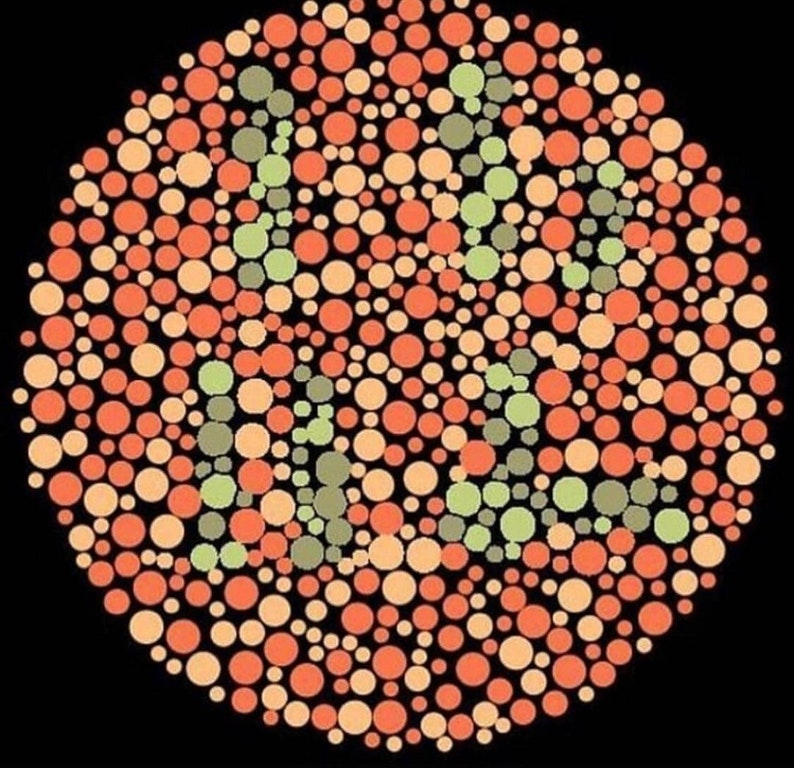
\includegraphics[height=3cm,width=3cm]{loss_color}
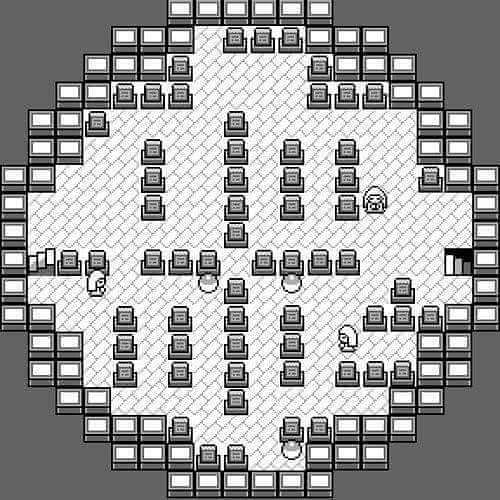
\includegraphics[height=3cm,width=3cm]{pokemon}
\caption{Edit basado en color (izq.) y en orientación (der.)}
\label{fig:color}
\end{figure}

\subsubsection{Problemas con detección de aristas}

Procesar las imágenes para obtener las aristas se consideró una propuesta poco
viable pues se tiene mucho ruido o se pierde información. Usando el modelo
\textsc{Canny} de \textsc{OpenCV} para obtener las aristas presentes en una imagen
nos encontramos con mucho ruido, por ejemplo, si un edit se construyó con fotografías
con muchos detalles en ellas y objetos innecesarios no fueron desenfocados, las
aristas de dichos objetos se extraen en conjunto con los polígonos que nos
interesan. Si modificamos los umbrales inferior y superior del modelo para filtrar
aristas podemos eliminar aristas de los objetos que nos interesan realmente. Estos
problemas se pueden apreciar en la Figura ~\ref{fig:canny}.

\begin{figure}[h]
\centering
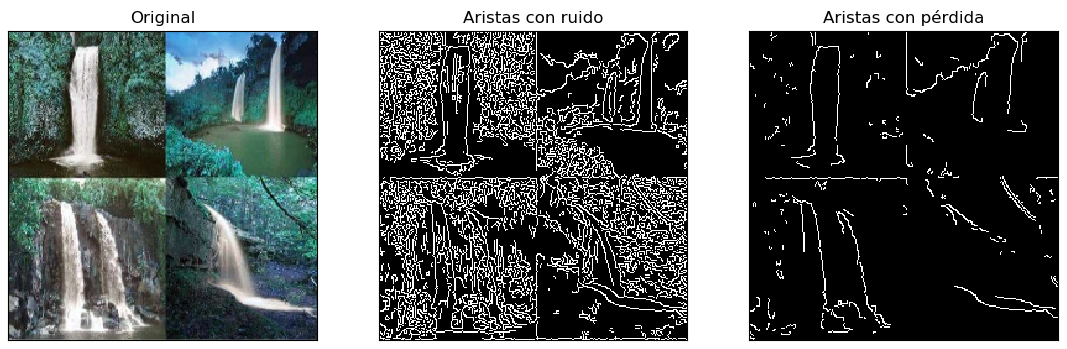
\includegraphics[width=0.8\textwidth]{edges}
\caption{Detección de aristas, algoritmo de Canny.}
\label{fig:canny}
\end{figure}

Además, los umbrales inferior y superior pueden no funcionar en distintas imágenes,
preservando ruido o perdiendo información. La baja resolución de las imágenes
también dificulta este proceso pues los bordes de los contenidos ya no son tan
finos como en la resolución original.

\subsection{Implementación}

La implementación se realizó en el lenguaje de programación \textsc{Python}%
\footnote{Versión 3.6.4, \url{http://www.python.org/downloads/release/python-364/}}.
Para la construcción de la red neuronal convolucional nos apoyamos de los
paquetes \textsc{TensorFlow}\footnote{\url{http://www.tensorflow.org/}} y
\textsc{Keras}\footnote{\url{http://keras.io}}.

Para nuestros modelos construimos 4 redes convolucionales con las siguientes
arquitecturas:

\begin{itemize}
\item Modelo 1. Trabaja con imágenes en escala de grises. Tiene 2 capas de convolución
con función de activación ReLU  32 filtros, la primera usa filtros de tamaño
$5 \times 5$ con pasos (\textit{strides}) de 3, la segunda filtros de tamaño
$3 \times 3$ con pasos de 2. La salida de cada capa pasa a una capa de max pooling
con ventanas de $2 \times 2$ que no se traslapan. Finalmente un perceptrón multicapa
con 2 capas ocultas de 64 nodos y activación ReLU y una capa de salida de un nodo
con activación la función sigmoide (clasificaión binaria). Para el entrenamiento
se usa el optimizador ADAM con función de pérdida entropía cruzada (\textit{Cross entropy}).
La red se entrenó durante 10 épocas en lotes de 32 imágenes.
\item Modelo 2. Exactamente lo mismo que el Modelo 1, pero trabajo con imágenes
a color RGB.
\item Modelo 3. El modelo 2 pero con optimizador ADAGRAD.
\item Modelo 4. Trabaja con imágenes a color RGB. Primera capa oculta con 128
filtros, pasos de 2; segunda capa oculta con 64 filtros y pasos de 1. Perceptrón
multicapa con arquitectura (256,128,1). Optimizador ADAGRAD. Todo los demás
parámetros son iguales.
\end{itemize}

\section{Resultados}

A continuación se presentan los resultados obtenidos por los 4 modelos al final
de las 10 épocas de entrenamiento. Al principio del entrenamiento los modelos
tienen una precisión al rededor de 50\% pues están adivinando al azar y la pérdida
suele ser elevada. Para comparación se agrega también los resultados obtenidos
tras la primera época.

\begin{center}
\begin{tabular}{|l||r|r|r|r|}
\hline
\multicolumn{5}{|c|}{Primera época}
\\ \hline
& \multicolumn{2}{|c|}{Entrenamiento} & \multicolumn{2}{|c|}{Verificación}
\\ \hline
Modelo & Precisión & Pérdida & Precisión & Pérdida
\\ \hline
Modelo 1 & 57.55\% & 0.6792 & 65.89\% & 0.6082\\
Modelo 2 & 59.53\% & 0.6497 & 75.64\% & 0.5496\\
Modelo 3 & 57.34\% & 0.7224 & 64.50\% & 0.6368\\
Modelo 4 & 53.81\% & 2.3251 & 58.00\% & 0.6743\\
\hline
\end{tabular}
\end{center}

\begin{center}
\begin{tabular}{|l||r|r|r|r|}
\hline
\multicolumn{5}{|c|}{Décima época}
\\ \hline
& \multicolumn{2}{|c|}{Entrenamiento} & \multicolumn{2}{|c|}{Verificación}
\\ \hline
Modelo & Precisión & Pérdida & Precisión & Pérdida
\\ \hline
Modelo 1 & 97.03\% & 0.0837 & 87.24\% & 0.3743\\
Modelo 2 & 97.33\% & 0.0756 & 86.54\% & 0.3986\\
Modelo 3 & 95.50\% & 0.1342 & 84.69\% & 0.3883\\
Modelo 4 & 93.24\% & 0.1753 & 87.94\% & 0.3416\\
\hline
\end{tabular}
\end{center}

\section{Conclusiones}

Podemos apreciar como los diferentes modelos no cambian mucho sus valores de precisión y pérdida, a pesar
de que el modelo sea significativamente mas grande que los otros modelos, el hecho de que se cambie de
optimizador o se utilice la escala de grises contra las imagenes con sus colores normales, no tienen una mejora
significativa.

Como conclusión nos atrevemos a decir que para una red neuronal convolusional tiene un buen desempeño en el
problema de reconocer si una imagen cumple con un patrón, en este caso siendo el meme de Loss el patrón a
reconocer.

\begin{thebibliography}{9}
\bibitem{haykin}
Haykin, S. S. (2011).
\textit{Neural networks and learning machines}.
New Dehli: PHI Learning.

\bibitem{wuj}
Wu, J. (2018).
\textit{Convolutional neural networks}.
National Key Lab for Novel Software Technology. Nanjing University, China.
Obtenido de \url{http://cs.nju.edu.cn/wujx/teaching/15_CNN.pdf}.

\bibitem{pooling}
Scherer, D., M\"uller, A., \& Behnke, S. (2010).
\textit{Evaluation of Pooling Operations in Convolutional Architectures for Object Recognition}.
Artificial Neural Networks-ICANN 2010 Lecture Notes in Computer Science, 92-101. DOI:10.1007/978-3-642-15825-4\_10.

\bibitem{lecun}
Lecun, Y., Bottou, L., Bengio, Y., \& Haffner, P. (1998).
\textit{Gradient-Based Learning Applied to Document Recognition}.
Proceedings of the IEEE, 86(11), 2278-2324. DOI:10.1109/5.726791.

\bibitem{limitations}
Hosseini, H., Xiao, B., Jaiswal, M., \& Poovendran, R. (2017).
\textit{On the Limitation of Convolutional Neural Networks in Recognizing Negative Images}.
arXiv:1703.06857. Obtenido de \url{https://arxiv.org/pdf/1703.06857.pdf}.

\bibitem{adagrad}
Ducji, J., Hazan, E., \& Singer, Y. (2011).
\textit{Adaptive Subgradient Methods for Online Learning and Stochastic Optimization}.
Journal of Machine Learning Research 12, 2121-2159.

\bibitem{adam}
Kingma, D. P. \& Lei Ba, J. (2014).
\textit{Adam: A Method for Stochastic Optimization}.
arXiv:1412.6980. Obtenido de \url{http://arxiv.org/pdf/1412.6980.pdf}.

\bibitem{loss}
\textit{Talking to the Man Behind `Loss,' the Internet's Longest-Running Miscarriage `Joke'}.
\url{http://nymag.com/selectall/2015/11/longest-running-miscarriage-meme-on-the-web.html}

\end{thebibliography}

\end{document}
